\section{Grundlagen}
\label{sec:grundlagen}

\subsection{Betrachtung von Erdöl}

Bei Erdöl handelt es sich um den wichtigsten Energieträger des 20. Jahrhunderts bis hin zur Gegenwart. Durch Erdöl wurden viele technologische Entwicklungen begünstigt oder gar erst möglich gemacht. Durch systematische Aufbereitung in Reffinerien sind neben den offensichtlichen Anwendungen wie der Nutzung als Schmier-- und Kraftstoff für Mobilität und Maschinen oder zur Wärmegewinnung sind viele weitere Anwendungen möglich, ohne die die moderne Gesellschaft nur schwer vorstellbar wäre\footnote{z.b. Kunststoffe und Lacke, welche zum großen Teil auf Erdöl basieren, oder auch die Reichweite, die Fahrzeuge wegen der hohen Energiedichte von Benzin bzw. Diesel erzielen.}.

Die Wertschöpfungskette rund um Erdöl gliedert sich in die Phasen des Finden bzw. Förderns, des Sammelns bzw. Aufbereitens und in die anschließende Nutzung in diversen Endprodukten, vom Treibstoff bis hin zu diversen Kunsstoffen.
Dabei gilt, dass Erdöl zwar in großen Mengen\footnote{Ob diese Mengen, speziell im Vergleich zum weltweiten Verbrauch, tatsächlich immer noch groß sind, wird z.T. bezweifelt}, aber nicht unbegrenzt zur Verfügung steht. 

Die Auswirkungen des Erdöls auf Technologie, Wirtschaft, Gesellschaft und Politik des 20. Jahrhunderts sind enorm. Erdöl ermöglichte großen Reichtum von Unternehmen und Staaten, aber verursachte auch Krisen und Kriege.

\subsection{Definition: Daten, Information, Wissen}
\label{defwissen}

In dieser Arbeit sollen die folgenden Definitionen gelten: Ein \buzz{Datum} ist eine formalisierte Sachverhaltsaussage, ohne inhärente Bedeutung (z.B. „23°C“). Durch Interpretation im Kontext kann daraus eine \buzz{Information} werden (z.B. „Die Außentemperatur beträgt 23°C“)\footnote{vgl. \cite{kfk}, Seite 40}. Durch Vernetzung mehrerer Informationen miteinander, aber auch durch Erfahrung kann \buzz{informatives Wissen} entstehen (z.B. „Das Wetter ist schön“)\footnote{vgl. \cite{pnik}, Seite 106}. 

In weiteren Verfeinerungsschritt entsteht dann \buzz{handlungsorientiertes Wissen}, (z.B. „Ich benötige beim Nachmittagsspaziergang keinen Pullover“) das dann zu einer konkreten Entscheidung führen kann (z.B. „Ich lasse den Pullover zu Hause.“)\footnote{vgl. \cite{taylor}, Seite 342}.

\subsection{Definition: Web 1.0, Web 2.0}

Unter \buzz{Web 1.0} versteht man das \ac{WWW} wie es ursprünglich entwickelt wurde: Eine Menge von statischen Daten, die miteinander auf willkürliche Weise verknüpft werden konnten. Die Auszeichnungssprache \ac{HTML} ermöglicht es Autoren, bestimmte Abschnitte zu kennzeichnen. Schon hier gibt es unterschiedliche Informationsgehalte der Auszeichnungen: Während \code{<b>…</b>} lediglich aussagt, dass der ausgezeichnete Abschnitt in fetter Schriftart angezeigt werden soll, ist eine mit \code{<h1>…</h1>} ausgezeichnete Überschrift tatsächlich als solche zu erkennen. Auch wenn die dadurch gewonnene Information für ein automatisch erstelltes Inhaltsverzeichnis schon nützlich sein kann, wird hier keine Aussage bzgl. des eigentlichen Inhalts getroffen. Somit sind die Dokumente des Web 1.0 dem Bereich der \buzz{Daten} zuzuordnen. Die darin enthaltenen Informationen bzw. das darin enthaltene Wissen ist erst zugänglich, wenn die Daten durch Menschen gelesen und ausgewertet werden\footnote{vgl. \cite{alkhatib}, Seite xvi}.

Durch die Technologien des \buzz{Web 2.0} werden die Daten i.d.R. in Datenbanken vorgehalten und die Webseiten erst bei Abruf generiert. Durch die Popularität von Werkzeugen wie Blogs und Wikis sind deutlich mehr Menschen an der Erstellung der Inhalte beteiligt. Weitere Daten werden durch Techniken rund um das \buzz{\ac{IoT}} und \buzz{Ubiquitous Computing} automatisch erfasst. Diese Daten mit sogenannten \buzz{Meta--Daten} angereichert. Hierdurch wird in maschinenlesbarer Form angegeben, welche Informationen die Dokumente enthalten. Neben vom Autor selbst zugeordneten \buzz{Tags} und \buzz{Kategorien} kommen auch automatisch generierte Meta--Daten hinzu. Beispiele hierfür sind etwa das Veröffentlichungsdatum, Beziehungen zu anderen Dokumenten\footnote{Realisiert durch sog. Backtracks -- Wer verlinkt auf dieses Dokument?} oder Geoinformationen (Wo wurde das Dokument erstellt). Inzwischen werden auch die Stimmung des Autors erfragt (z.B. bei Runtastic–Aktivitäten) oder ermittelt (z.B. bei Facebook--Einträgen). Die durch Daten und Meta--Daten erzielte Informationsstufe ist deutlich über der von \buzz{Web 1.0}, unterliegt aber deutlichen Schwankungen je nach Dienst bzw. Nutzereingaben.

\subsection{Web 3.0 = Web 2.0 + Semantik = Semantisches Web}

„\buzz{Semantik}, auch \buzz{Bedeutungslehre}, nennt man die Theorie oder Wissenschaft von der Bedeutung der Zeichen. Zeichen können in diesem Fall Wörter, Phrasen oder Symbole sein. Die Semantik beschäftigt sich typischerweise mit den Beziehungen zwischen den Zeichen und den Bedeutungen dieser Zeichen.“\footnote{cite{wp:semantik}}

Im \buzz{Web 3.0} werden die Daten bzw. Informationen des Web 2.0 durch Beifügung von Bedeutung zu Information bzw. informativem Wissen veredelt\footnote{vgl. \cite{nyt:markoff}}. Hierdurch soll es möglich werden, die schnell steigenden Datenmengen sinnvoll zu nutzen\footnote{vgl. \cite{tsp:tolksdorf}}. Die Bezeichnung \buzz{semantisches Web} ermöglicht eine Abgrenzung gegenüber anderen Interpretationen des Buzzwords \buzz{Web 3.0}, wie sie z.T. im Marketing\footnote{z.B. „Web 3.0 marketing is the convergence of new technologies and rapidly changing consumer buying trends.“ in \cite{web3market}, Abschnitt „What is Web 3.0 Marketing?“} oder in der Politikwissenschaft\footnote{z.B. „Is this Web 3.0? Not a tech-upgrade, a smarter algorithm, slicker fibre optic or better Bluetooth beam. Instead, Web 3.0 as in an outcome, the demonstrated consequences of being able to access information?“ in \cite{web3pol}, Abschnitt „Web 3.0: Regime Change“} zu finden sind.

\subsection{Die Bedeutung der Daten}

Den vorhandenen oder neu gesammelten Daten kann auf verschiedene Arten Bedeutung beigefügt werden. Sogenannte \buzz{Meta--Daten} beschreiben Dateien durch Schlagworte oder Zuordnung von Werten zu definierten Schlüsselworten. Die Meta--Daten können in seperaten Dateien gespeichert werden\footnote{z.B. in den .INFO--Dateien in der Benutzeroberfläche des Comodore Amiga „Workbench“, oder in der Bilderdatenbank der Applikation „Adobe Lightroom“}. Ebenfalls möglich ist die Speicherung direkt in der entsprechenden Datei\footnote{z.B. EXIF--Daten in Bilddateien oder Informationen zum Werk in MP3--Dateien}. Diese Daten werden i.d.R. automatisch\footnote{z.B. durch die Kamera beim fotografieren.} oder halbautomatisch\footnote{Einmalig manuell, dann Bereitstellung für andere Nutzer per CDDB oder andere Dienste.} den Daten zugeordnet. Manche Metadaten können auch bei Abruf direkt ermittelt werden\footnote{z.B. Dateigröße}.

In textbasierten Dateiformaten wie XML werden hingegen einzelne Elemente durch Markup--Tags maschinenlesbar mit Bedeutung versehen werden. So werden Zeichenketten als Namen, Adressen, Telefonnummer etc. identifizier-- und auswertbar. Die Meta--Daten sind hier Teil des Datenstroms.

Durch Techniken wie Gesichtserkennung oder Textanalyse können Meta--Daten auch automatisch aus den Daten generiert werden. Hierbei bestimmt die Menge der auszuwertenden Daten und die Qualität der bereits vorhandenen Metadaten die Qualität der Ergebnisse.

Durch Regelwerke, hinterlegte Logik, Verknüpfungen und standardisiertem Datenaustausch können aus den Informationen auch Wissen erzeugt werden:
Person A ist auf einem Bild zusammen mit Person B zu sehen (Gesichtserkennung). Die Geoinformation und Uhrzeit (EXIF--Tags) zeigen, dass das Foto auf einer Veranstaltung aufgenommen wurde, das zu diesem Zeitpunkt an diesem Ort statt fand (Semantisches Markup der Veranstaltung).
Daraus kann auf politische Gesinnung, Musikgeschmack und/oder Trinkfreudigkeit von Person A geschlossen werden.

\begin{figure}[H]
\begin{center}
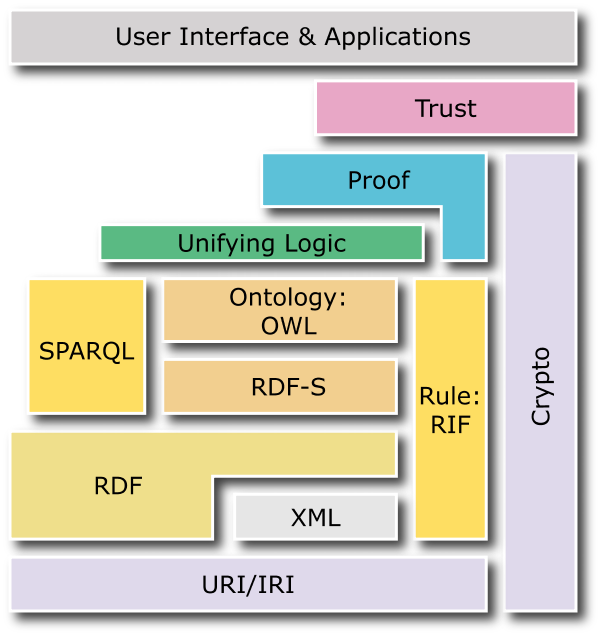
\includegraphics[width=0.4\textwidth]{layerCake-4.png}
\caption{Der Stack des semantischen Web}
\label{pic:tsemanticstack}
\end{center}
\end{figure}